 % mainfile: ../../../../master.tex
\label{task:20240416_aosp}

\subsection{ART Loading Process of Classes and Methods}

\subsubsection{Find the number of target DEX class in the DEX file}

Need to get the corresponding OAT class in the OAT file using the number of target DEX class.

\begin{longtable}{p{.30\linewidth}p{.60\linewidth}} 
\toprule
 Procedure & Description \\
\midrule
\endhead

\multicolumn{2}{l}{\path{frameworks/base/core/jni/AndroidRuntime.cpp}}\\

\path{AndroidRuntime::start}
&
\\
\path{AndroidRuntime::startVm}
&
\\

\midrule
\multicolumn{2}{l}{\path{art/runtime/jni/java_vm_ext.cc}}\\

\path{JNI_CreateJavaVM}
&
\\

\midrule
\multicolumn{2}{l}{\path{art/runtime/runtime.cc}}\\

\path{Runtime::Create}
&Before starting ART, you have to first create ART virtual machine, which will be used to start Zygote Process which runs System Server and Android Apps.
\\
\path{Runtime::Init}
&Parses and parameters for the startup of ART (if image file (an OAT file contianing multiple DEX files) is not specified, \path{/system/framework/boot.art} will be prepared in advance in the system partition to be used as ART virtual machine); create an ART Heap based on the parameters
\\

\midrule
\multicolumn{2}{l}{\path{art/runtime/thread.h}}\\

\path{GetJniEnv}
&Get APIs to ART Java VM of current running thread. The APIs are wrapped in \texttt{struct JNIEnvExt} which is an extension of \texttt{JNIEnv}, and stores \texttt{JNINativeInterface}.
\\

\midrule
\multicolumn{2}{l}{\path{libnativehelper/include_jni/jni.h}}\\

\path{JNIEnv}
&Wraps functions to call ART Java VM to execute Java classes and methods.
\\
\path{JNINativeInterface}
&Wraps functions to call ART Java VM to execute Java classes and methods. Among them is \texttt{JNI::FindClass} which is defined in \path{art/runtime/jni/jni_internal.cc}.
\\

\midrule
\multicolumn{2}{l}{\path{art/runtime/jni/jni_internal.cc}}\\

\path{FindClass}
&Check if runtime instance has started, and then calls \texttt{ClassLinker}'s \texttt{FindClass}. If not started, calls \texttt{ClassLinker}'s \texttt{FindSystemClass} (which also calls \texttt{ClassLinker}) instead.
\\

\midrule
\multicolumn{2}{l}{\path{art/runtime/class_linker.cc}}\\

\path{ClassLinker::FindClass}
&
\\
\path{ClassLinker::LookupClass}
&Check whether the class has already been loaded. If so, just return the corresponding class object.
\\
\path{ClassLinker::FindInClassPath}
&Find the class in DexFile, if \path{class_loader} is null. Then call \texttt{ClassLinker::DefineClass} to load the class from the loaded DEX.
\\
\path{ClassLinker::DefineClass}
&Use the \path{class_loader} object (of \texttt{java.lang.ClassLoader} type) to load the specified class. For system classes
\\

\midrule
\multicolumn{2}{l}{\path{art/runtime/jni/jni_env_ext.cc}}\\

\path{GetJniEnv}
&Get APIs to ART Java VM of current running thread. The APIs are wrapped in \texttt{struct JNIEnv}.
\\

\midrule
\multicolumn{2}{l}{\path{art/runtime/thread.h}}\\

\path{GetJniEnv}
&Called by \path{JNI_CreateJavaVM}
\\

\path{Thread::Attach}
&Parses and parameters for the startup of ART (if image file (an OAT file contianing multiple DEX files) is not specified, \path{/system/framework/boot.art} will be prepared in advance in the system partition to be used as ART virtual machine); create an ART Heap based on the parameters
\\

\midrule
\caption{Class Loading Process} 
\label{tab:classloadingprocess}
\end{longtable}

\subsubsection{Repeat the same steps for DEX Method}

\subsubsection{Calculate local machine instructions for the methods}

\subsection{ART Execution Process of Classes and Methods}

\subsection{ART Java VM}

\subsubsection{Which components are involved in Framework for Debloation?}
\subsection{Find Links on Permission Manager}
\subsection{Find Links on Package Manager}
\subsection{Explore Package Manager Service Source Codes}
\subsection{Complete Package Manager Loading Flow}
\subsection{Instrument Package Manager Process}
\subsection{Understand Zicheng's Changes to Package Manager}

\subsection{Intersection between ART/Bionic/Framework and Debloater Procedures}

\subsection{Debloater Procedures not included in OAT/Classes Loading and Execution Flow}

\subsection{Sequence Diagram Debloater Flow}

\subsection{Instrument Debloater Flow}

\subsection{Instrument ART Native Execution Flow}

\subsection{Instrument ART Interpreted Execution Flow}

\subsection{Implement Rudimentary Hardcoded Debloater in AOSP 13}

\subsection{Implement Rudimentary Hardcoded Debloater in AOSP 14}


% 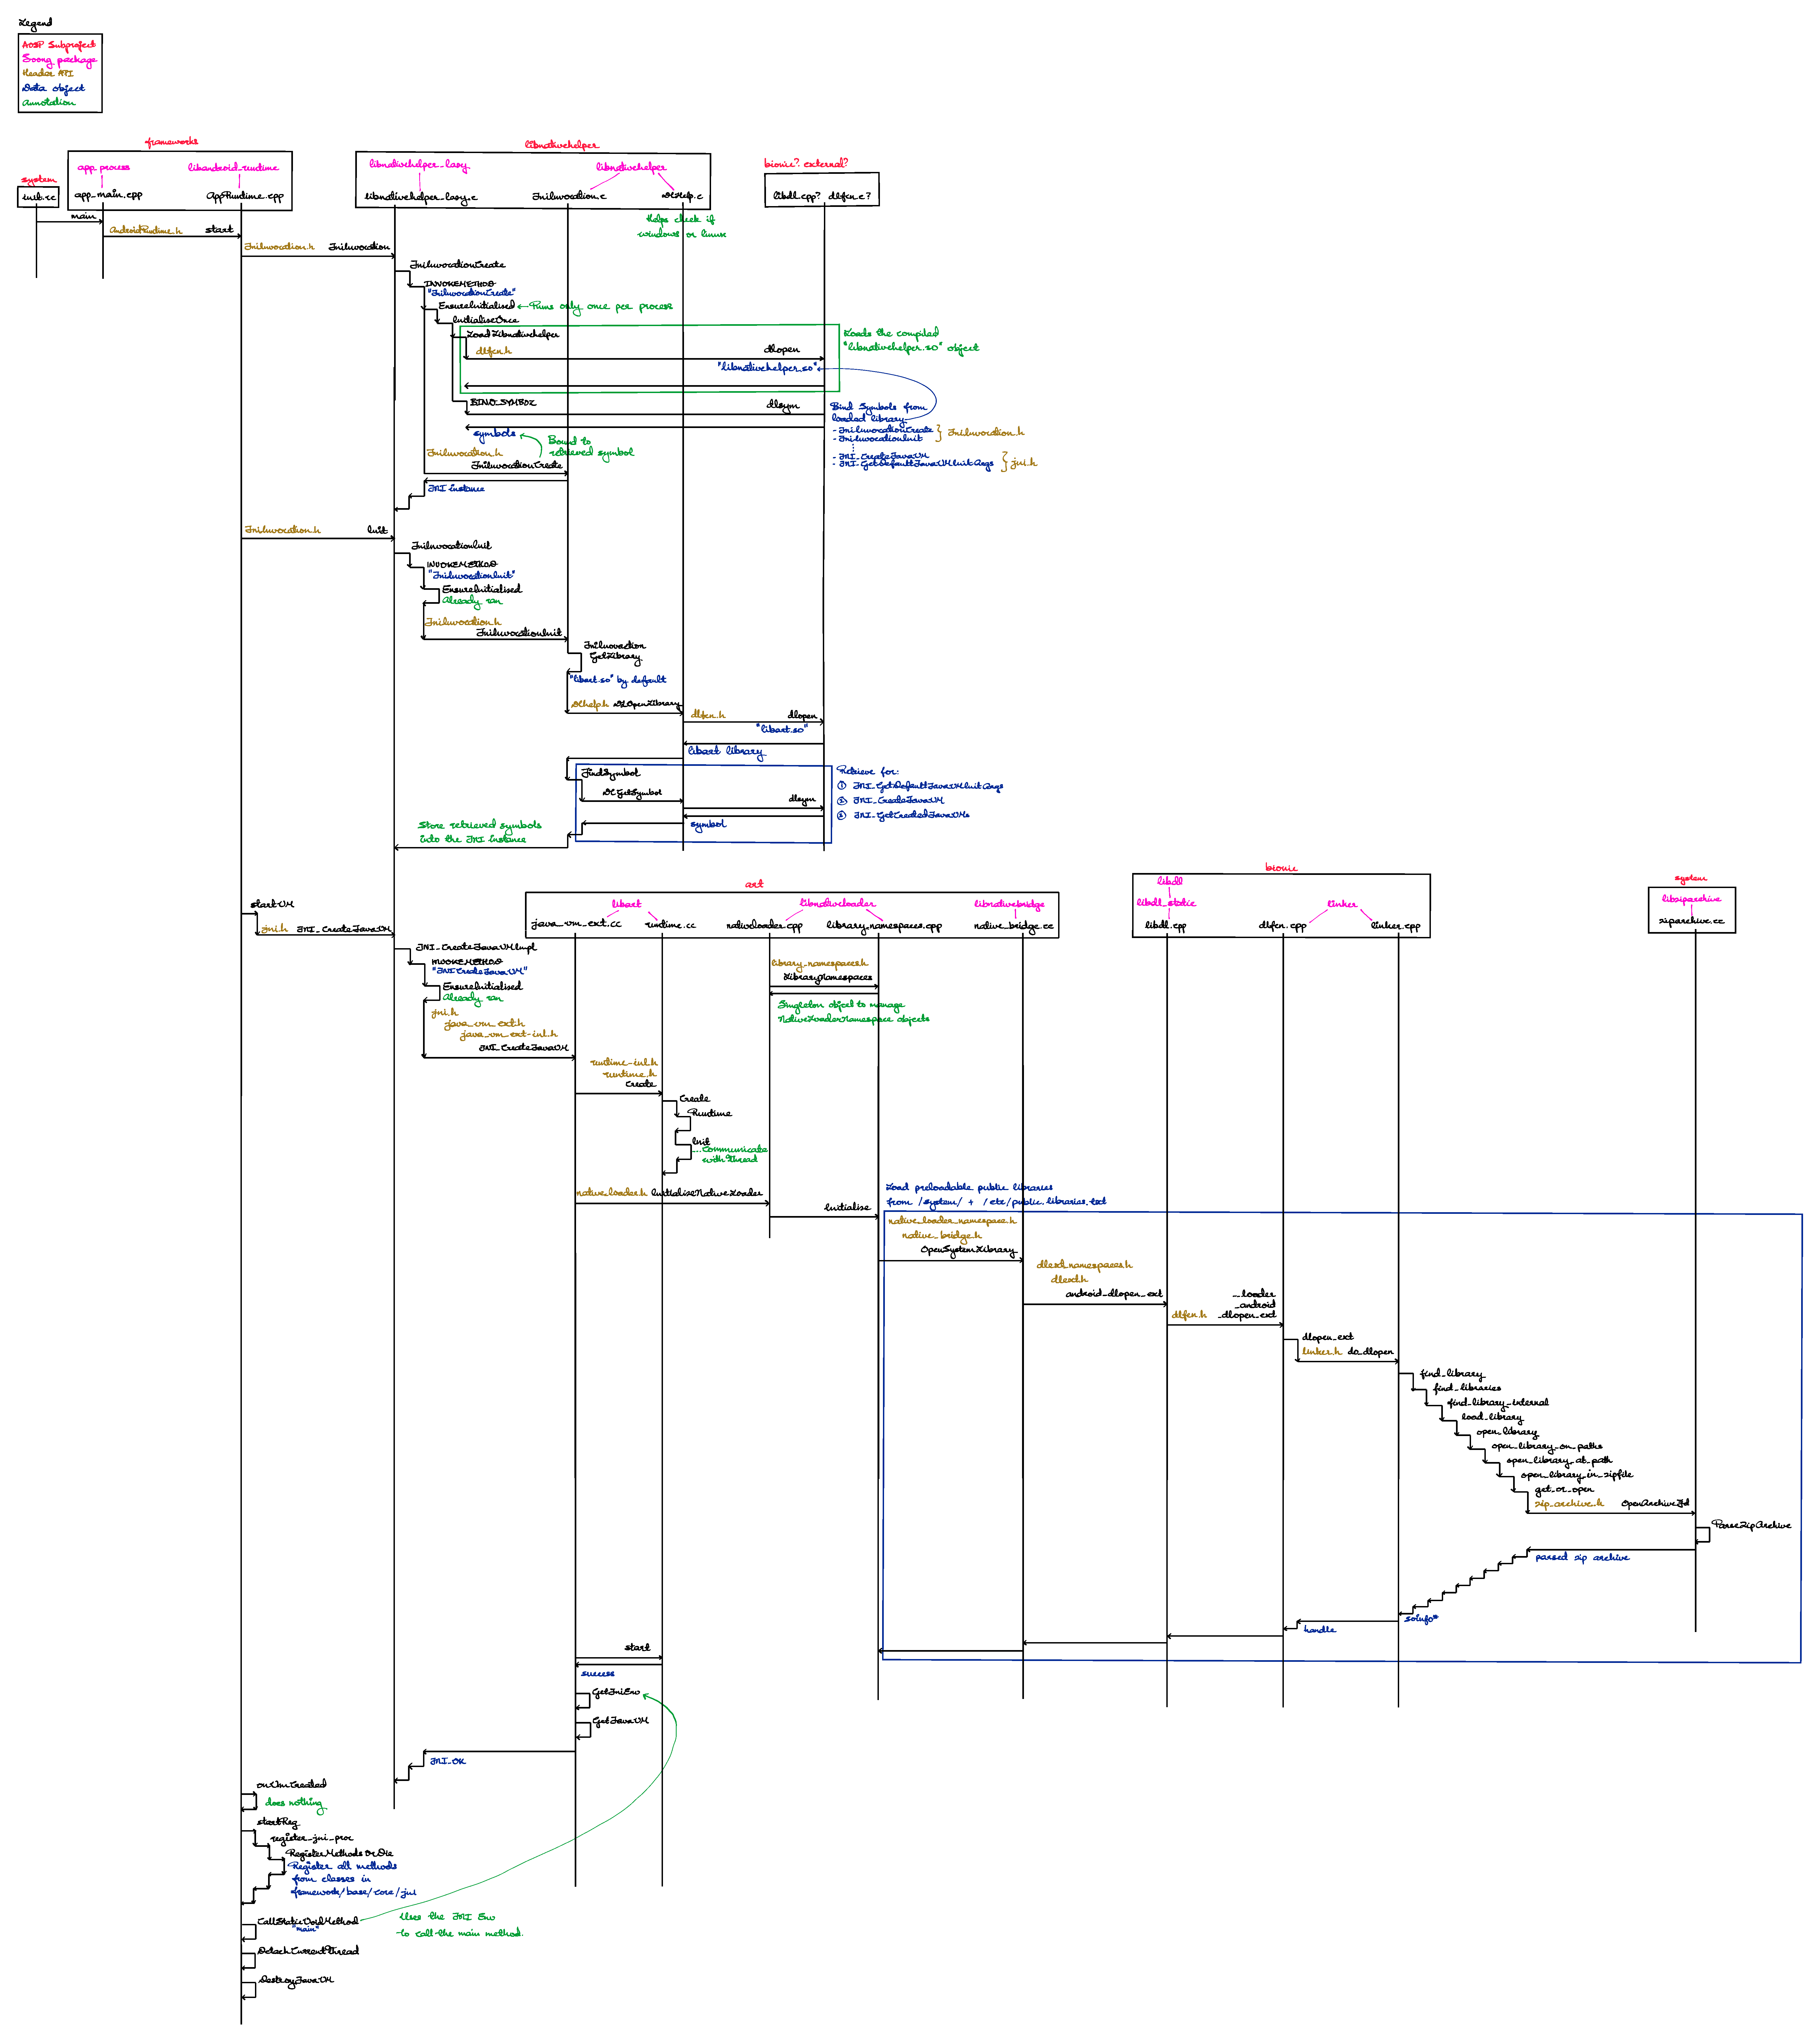
\includepdf[pages=-, scale=.95,pagecommand={}]{entries/2024/01/01/art.pdf}

% \begin{itemize}
% \item \textbf{Domain.} The context of the process that is acting upon something.
% \item \textbf{Type.} The context of the resource on which the process is acting.
% \item \textbf{Class.} The object class of the resource (e.g. \textit{file} or \textit{socket}).
% \item \textbf{Permissions.} The permissions that are allowed given the \textit{domain}, \textit{type} and \textit{class}.
% \end{itemize}

% SELinux rule syntax:


% \subsubsection{Decoding Permission Denial Message}

% Message:
% \begin{lstlisting}
% type=AVC msg=audit(1363289005.532:184): avc:  denied  { read } for  pid=29199 comm="Trace" 
% name="online" dev="sysfs" ino=30 scontext=staff_u:staff_r:googletalk_plugin_t 
% tcontext=system_u:object_r:sysfs_t tclass=file
% \end{lstlisting}

% \begin{longtable}{p{.15\linewidth}p{.15\linewidth}p{.65\linewidth}} 
% \toprule
% Log part & Name & Description \\
% \midrule
% \endhead

% \texttt{type=AVC}
% &Log type
% &Only in the \texttt{audit.log} file; it informs the user what kind of audit log type this is. 
% \\

% \midrule
% \caption{Permission Denied Syntax} 
% \label{tab:permissiondeniedsyntax}
% \end{longtable}


% \subsubsection{SELinux Architecture}

% SELinux consists of four main components: object managers (OM), access vector cache (AVC), security server, and security policy as show below:
% \begin{figure}[H]
%     \centering
%     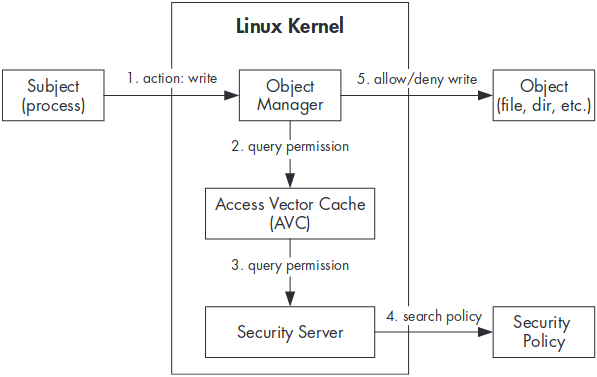
\includegraphics[width=.85\linewidth]{entries/2023/12/10/selinux.png}
%     \caption{SELinux Components}
%     \label{fig:selinux}
% \end{figure}
